\section{Data and Methodology} \label{sec:methodsanddata}

This section describes the data and estimation strategy. Section \ref{sec:data} describes the data in detail. Section \ref{sec:descriptive} presents descriptive evidence. Section \ref{sec:empiricalstrategy} details the estimation strategy used in this paper, contrasting it with the estimator I attempted to approximate and showing where the analysis remains limited. Finally, Section \ref{sec:identification_threats} discusses threats to identification.

\subsection{Data} \label{sec:data}

The main outcome data come from the São Paulo State School Performance Assessment System (SARESP), made available by the São Paulo State Department of Education.\footnote{The full databases are available at the Education Open Data portal: \url{https://dados.educacao.sp.gov.br/}.} SARESP is an annual assessment administered in almost all schools in the state system, measuring proficiency in Portuguese Language and Mathematics. This paper uses 9th grade of elementary school and the 3rd grade of high school, two stages that are comparable over the period analyzed and relevant for assessing the accumulated effects of the policy. SARESP has its own classification of proficiency levels; the details are available in the original monograph appendix.

The unit of analysis is the school-year-grade-subject panel. This choice follows from the available administrative structure: enrollment microdata allow me to characterize school composition, but they do not reliably link each enrolled student to her individual SARESP score. This occurs because the way student identifiers are coded in the outcomes database differs from the coding used in the enrollment database. Therefore, the main estimation is aggregated at the school level, although it is informed by statistics constructed from the microdata.

The main window runs from 2011 to 2018. The year 2011 provides the period immediately before PEI began in 2012. The upper limit of 2018 preserves a pre-pandemic window and avoids the comparability break associated with COVID-19 and the interruption of SARESP in 2020. Schools that joined PEI only after 2018 are treated as not-yet-treated within the main window.

The outcome is average school proficiency in each year, grade, and subject. To facilitate comparisons across years, scores are standardized within each year:

\begin{equation}
Y_{it}^{std} = \frac{Y_{it} - \bar{Y}_{t}}{\operatorname{sd}(Y_t)},
\end{equation}

where $Y_{it}$ is the average proficiency of school $i$ in year $t$, $\bar{Y}_{t}$ is the annual mean, and $\operatorname{sd}(Y_t)$ is the annual standard deviation. Estimated coefficients can therefore be interpreted in standard deviations of the annual proficiency distribution.

In addition to the proficiency panel, the paper uses enrollment microdata to construct aggregate composition covariates by school, year, and grade. These covariates include the share of female students, the share of students with a registered special need, average age, the share of Black or mixed-race students, the share of students with declared race/color, the share of Bolsa Familia beneficiaries, and school size measured by enrollment. The special-needs variable is an indicator equal to one when the administrative record reports any disability or specific educational condition. The data dictionary includes the following categories: multiple disability, blindness, low vision, severe or profound deafness, deafblindness, physical disability associated with cerebral palsy, physical disability-wheelchair user, Down syndrome, intellectual disability, monocular vision, childhood autism, Asperger syndrome, Rett syndrome, childhood disintegrative disorder, and giftedness.

When necessary, missing values in composition covariates are imputed using annual means. This choice preserves panel coverage and avoids making the main estimation depend only on schools with more complete administrative records. Section \ref{sec:results} presents a sensitivity diagnostic without imputation to document the sample cost of this decision.

This construction reflects the main empirical limitation of the paper. The microdata are not used to estimate individual PEI effects, because the link between enrollment and individual scores is not reliable over the relevant period. The enrollment and SARESP outcome databases do not share the same student identifier, preventing a direct merge that would perfectly control for migration effects. Such a merge would only be possible with authorized administrative access from the Department of Education, as in \textcite{scorzafave2023}. In this paper, the microdata enter as a source of aggregate covariates, allowing me to approximate observable compositional changes at the school level, but not at the student level.

I also incorporate municipal controls from local-characteristics databases made available by IBGE.\footnote{Available at \url{https://www.ibge.gov.br/estatisticas/economicas/contas-nacionais/9088-produto-interno-bruto-dos-municipios.html} and \url{https://www.ibge.gov.br/estatisticas/sociais/populacao/9103-estimativas-de-populacao.html}.} The municipal covariates are municipal GDP per capita, total municipal population, and the share of the population aged 0 to 19.

\subsection{Descriptive Evidence} \label{sec:descriptive}

Before the causal estimation, Figures \ref{fig:notas9ano} and \ref{fig:notas3ano} show the evolution of average SARESP scores by school stage. They indicate that schools that join PEI experience proficiency growth after conversion. This evidence is useful for visualizing the basic pattern in the data, but it does not identify the causal effect of the program. The observed increase may reflect learning, pre-existing differences across schools, selection into the program, and changes in the composition of assessed students.

\begin{figure}[htbp]
    \centering
    \caption{Evolution of SARESP scores - 9th grade}
    \label{fig:notas9ano}
    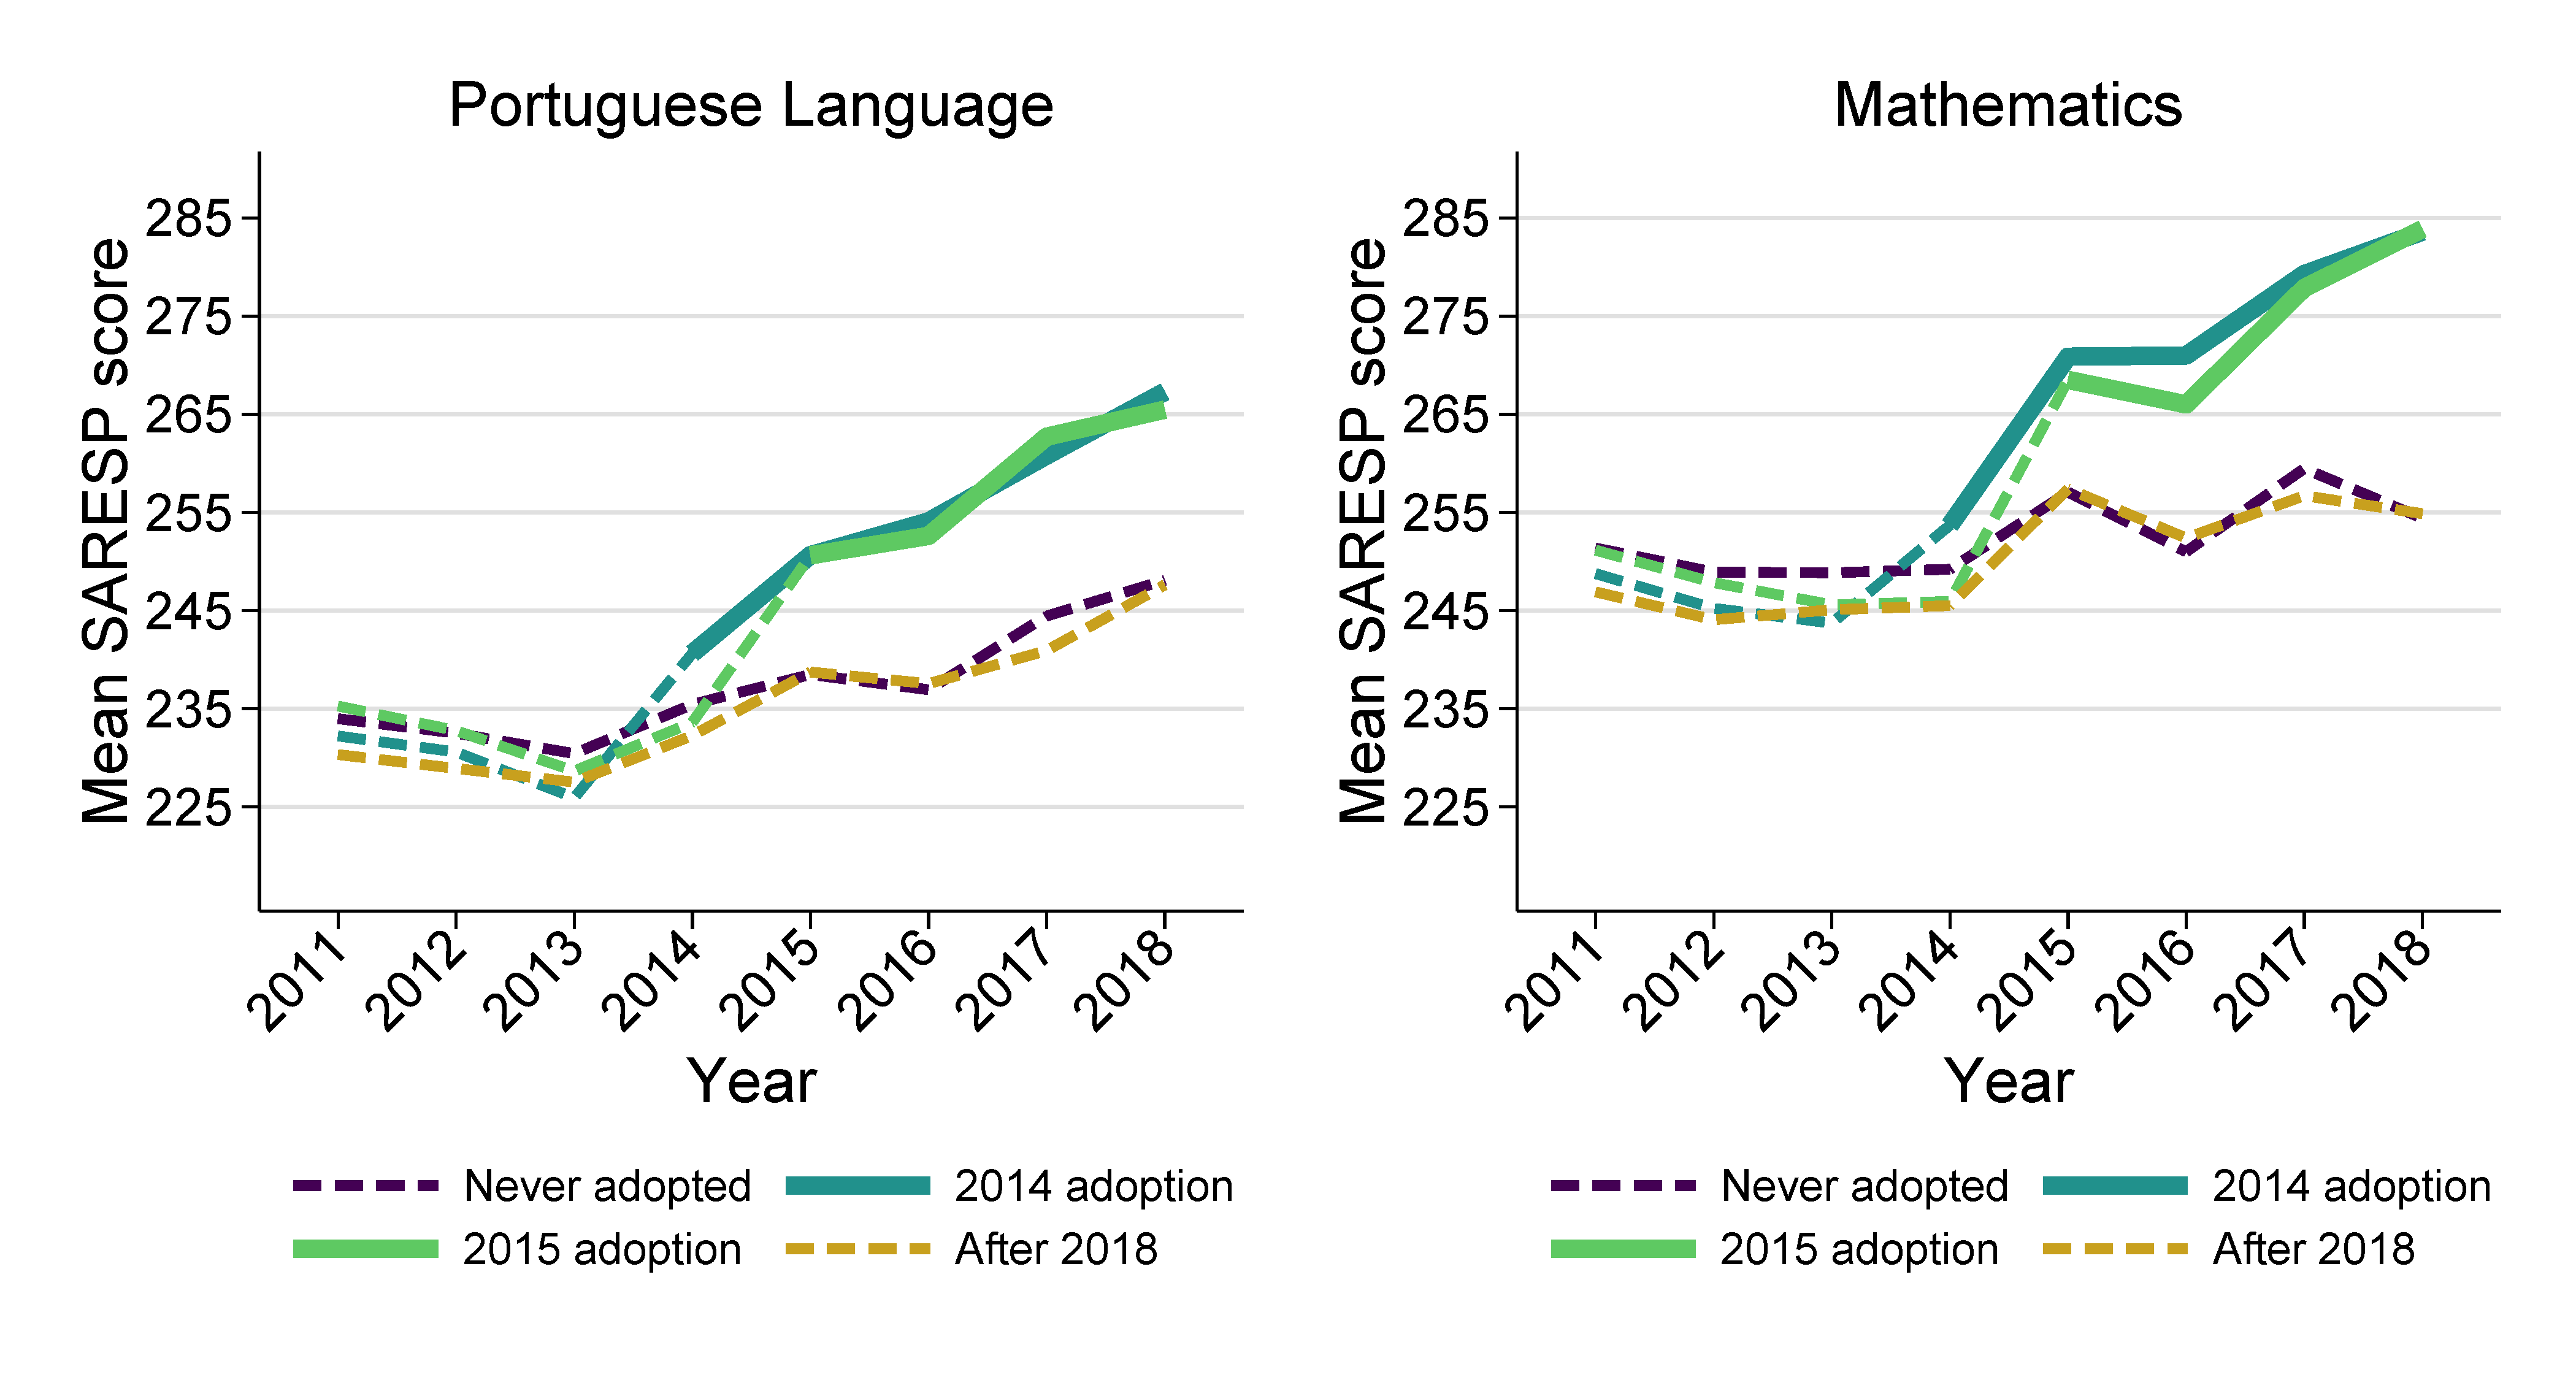
\includegraphics[width=1\textwidth]{files/images/medias_ef9_combine.pdf}
    \caption*{\footnotesize \textit{Source:} \href{https://dados.educacao.sp.gov.br/story/saresp}{Education Open Data}, author's elaboration.}
\end{figure}

\begin{figure}[htbp]
    \centering
    \caption{Evolution of SARESP scores - 3rd grade of high school}
    \label{fig:notas3ano}
    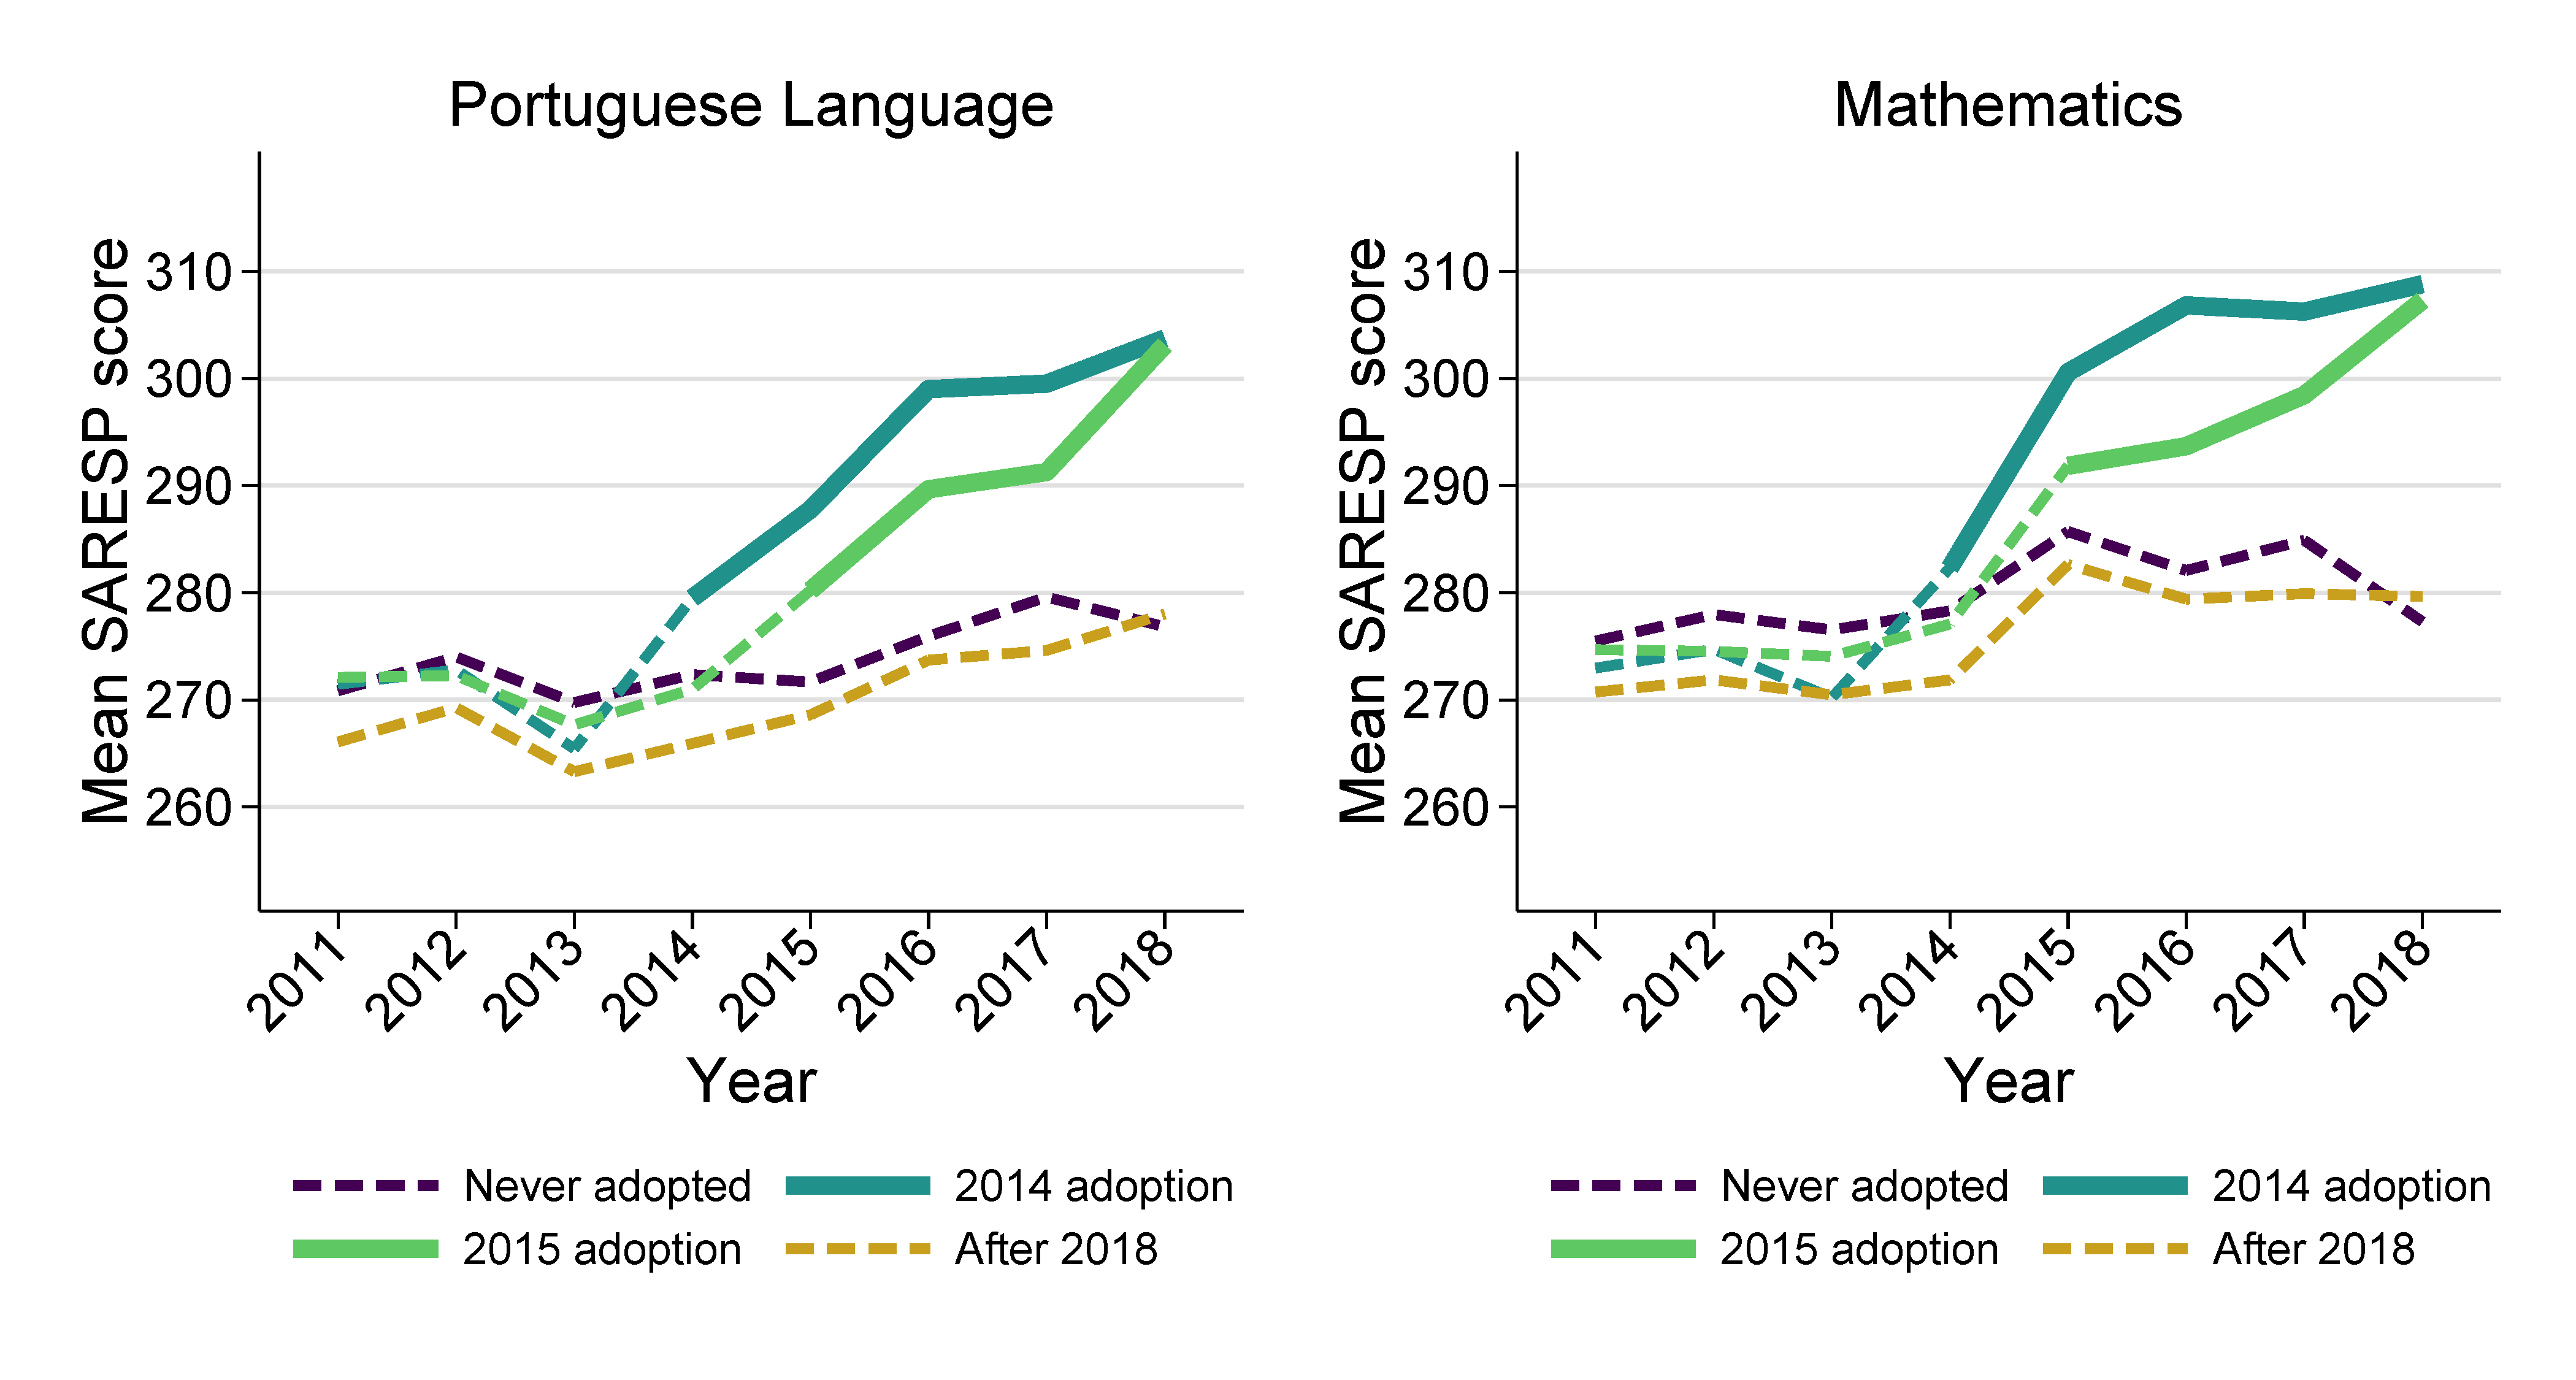
\includegraphics[width=1\textwidth]{files/images/medias_em3_combine.pdf}
    \caption*{\footnotesize \textit{Source:} \href{https://dados.educacao.sp.gov.br/story/saresp}{Education Open Data}, author's elaboration.}
\end{figure}

The figures also help interpret the scale of the problem. In absolute terms, PEI schools appear to move toward higher levels of proficiency, especially in high school. However, visual comparisons of raw means do not separate the direct pedagogical channel from the compositional channel. A school may improve because it teaches better, but also because it begins to receive, retain, or assess a different set of students. This distinction is precisely what motivates the empirical strategy below.

For this reason, in the main estimation proficiency is standardized by year and the effects are interpreted in standard deviations. This choice prevents changes in the annual SARESP scale or distribution from contaminating comparisons across periods. The empirical object is not only whether the mean of PEI schools increased, but whether this increase remains when compared with not-yet-treated or never-treated schools in a structure compatible with staggered adoption.

\subsection{Empirical Strategy} \label{sec:empiricalstrategy}

The empirical strategy exploits the staggered adoption of PEI across São Paulo state schools. Let $G_i$ be the first year in which school $i$ joins the program. The basic parameter of interest is the average treatment effect for cohort $g$ in period $t$:

\begin{equation}
ATT(g,t) = E\left[Y_{it}(g) - Y_{it}(0) \mid G_i=g\right], \quad t \geq g,
\end{equation}

where $Y_{it}(g)$ is the potential outcome of the school if treated from year $g$ onward, and $Y_{it}(0)$ is the potential outcome without treatment. The central problem is that $Y_{it}(0)$ is not observed for schools that have already converted. Identification therefore depends on constructing a plausible counterfactual using schools that have not yet joined or that do not join the program within the analysis window.

Table \ref{tab:estimadores} summarizes the progression of estimators used in the paper. The logic is not to present four equivalent answers. The sequence starts from a traditional benchmark, corrects the staggered-adoption problem, adds observable covariates, and finally tests the sensitivity of the results to compositional change.

\begin{table}[htbp]
\centering
\caption{Role of the estimators in the empirical strategy}
\label{tab:estimadores}
\small
\begin{threeparttable}
\begin{tabular}{p{2.4cm}p{3.3cm}p{3.7cm}p{3.5cm}}
\toprule
Estimator & Comparison used & What it corrects & Main limitation \\
\midrule
TWFE & Event study with school and year fixed effects & Fixed differences across schools and common year shocks & May make forbidden comparisons under staggered adoption \\
CS21 & $ATT(g,t)$ by cohort and period & Heterogeneous effects and staggered adoption & Does not by itself correct compositional change in RCS data \\
DR-DiD & $ATT(g,t)$ with outcome regression and weighting & Observable covariates and double robustness & Depends on the available aggregate covariates \\
S\&X approx. & 2x2 cells by cohort and relative time, with four-category multinomial logit & Sensitivity to observable composition at the aggregate level & Does not replace the individual estimator with linked student-score data \\
\bottomrule
\end{tabular}
\begin{tablenotes}
\footnotesize
\item \textit{Note:} The last row is not the literal implementation of the individual-level estimator of \textcite{santannaxu}; it is an aggregate approximation adapted to the absence of a reliable link between individual enrollment and individual scores.
\end{tablenotes}
\end{threeparttable}
\end{table}

From this point on, $i$ indexes schools, not students as in the microeconomic model in Section \ref{sec:micromodel}. The first specification is an event study with school and year fixed effects. Let $k=t-G_i$ denote relative time to conversion; $\alpha_i$ represents school fixed effects, $\lambda_t$ represents year fixed effects, and $X_{it}$ contains aggregate covariates used as controls:

\begin{equation}
Y_{it}^{std} = \alpha_i + \lambda_t + \sum_{k \neq -1} \beta_k \mathbb{I}\{t - G_i = k\} + X_{it}'\gamma + \varepsilon_{it}.
\end{equation}

This specification is useful as a reference, but it is not the preferred estimator. When adoption is staggered and treatment effects are heterogeneous over time, TWFE may compare already-treated schools with schools treated later, assigning weights to the average effect that are difficult to interpret.

The second specification uses the estimator of \textcite{callawaysantanna}. The method separately estimates $ATT(g,t)$ for each cohort and period, using not-yet-treated or never-treated schools as the comparison group. This prevents schools already exposed to PEI from serving as controls for schools treated later. The dynamic aggregation of these effects generates event-study coefficients, interpreted as average effects by relative time to conversion.

The third specification incorporates covariates through the doubly robust estimator associated with \textcite{santannazhao}. The intuition is to combine two ways of constructing the counterfactual. The first is an outcome model, which adjusts for observable differences across schools. The second is a propensity model, which reweights control units to make them more similar to treated units. If at least one of these components is correctly specified, the estimator preserves desirable asymptotic properties. In this paper, the covariates include baseline proficiency, municipal controls, and aggregate composition measures constructed from enrollment microdata.

The fourth specification is the most important adaptation in this paper. \textcite{santannaxu} show that, in repeated cross-sections, usual DiD identification may fail when treatment changes the composition of observed individuals. Their original proposal models the distribution of individual covariates and constructs counterfactuals that accommodate compositional changes. In applications of this type, this involves estimating probabilities of belonging to groups and periods, for instance through multinomial logits, and using weighting or matching to compare similar individual distributions.

The data design in this paper prevents a literal implementation. I do not observe, in the same reliable record, individual enrollment and individual SARESP scores. Therefore, I cannot estimate the model at the student level or perform individual matching between treated and control students based on the same set of characteristics and outcomes. The adaptation shifts the problem to the school-year-grade level. It does not perfectly decompose learning and selection, but it tests whether incorporating observable composition changes the estimated effect.

For each cohort $g$ and relative time $k$, I construct a 2x2 comparison using years $g-1$ and $g+k$. Define $D_i=1$ for schools in cohort $g$ and $T_i=1$ for observations in period $g+k$. This generates four cells:

\begin{equation}
(D_i,T_i) \in \{(0,0),(0,1),(1,0),(1,1)\}.
\end{equation}

Cell $(1,1)$ contains treated schools in the post-treatment period; $(1,0)$ contains the same schools in the period immediately before conversion; $(0,1)$ and $(0,0)$ contain control schools in the same years, respectively. The first step is to estimate a multinomial logit for the probability of each cell conditional on baseline covariates:

\begin{equation}
p_{dt}(X_i)=Pr(D_i=d,T_i=t \mid X_i), \quad d,t \in \{0,1\}.
\end{equation}

Covariates $X_i$ are fixed in year $g-1$, before cohort conversion. This choice avoids turning post-treatment characteristics into bad controls. In the implementation, I use the composition covariates with the best support in the aggregate panel: share of female students, average age, share of Black or mixed-race students, share of Bolsa Familia beneficiaries, and log enrollment. The variables are standardized within each 2x2 cell to improve the numerical stability of the multinomial logits.

From these probabilities, I construct Hajek weights for each cell. The operator $E_n[\cdot]$ denotes the sample mean and, in the denominator below, normalization is carried out within cell $(d,t)$:

\begin{equation}
w_{dt}(D_i,T_i,X_i)=
\frac{\mathbb{I}\{D_i=d,T_i=t\}\,p_{11}(X_i)/p_{dt}(X_i)}
{E_n[p_{11}(X_i)/p_{dt}(X_i) \mid D_i=d,T_i=t]}.
\end{equation}

These weights reweight the other cells to the observable distribution of the treated post-treatment cell, $(1,1)$. I then estimate three outcome regressions, one for each required counterfactual cell:

\begin{equation}
m_{dt}(X_i)=E[Y_i \mid D_i=d,T_i=t,X_i], \quad (d,t)\in\{(1,0),(0,1),(0,0)\}.
\end{equation}

The aggregate estimator inspired by S\&X combines weighting and outcome regression. For each pair $(g,k)$, the estimated function is:

\begin{equation}
\widehat{\tau}_{gk}^{SX} =
E_n\left[
w_{11}(Y-m_{10}-m_{01}+m_{00})
-w_{10}(Y-m_{10})
-w_{01}(Y-m_{01})
+w_{00}(Y-m_{00})
\right].
\end{equation}

The interpretation is direct: the first component uses the treated post-treatment cell, while the remaining components adjust the counterfactual evolution using the other three cells. The effects $\widehat{\tau}_{gk}^{SX}$ are then aggregated by relative time, with weights proportional to the number of treated schools observed in each post-treatment cell.

This form is the augmented version of the 2x2 difference-in-differences. If the regression terms were omitted, the estimator would collapse to the weighted difference $E_n[w_{11}Y]-E_n[w_{10}Y]-E_n[w_{01}Y]+E_n[w_{00}Y]$. The terms $m_{dt}(X_i)$ recenter each counterfactual cell through outcome regression, preserving the DiD intuition while adding adjustment for observable covariates.

This procedure required an important common-support restriction. Because treated schools account for a small share of the sample, some cells generate $p_{11}(X_i)$ probabilities very close to zero for a large share of controls. An initial attempt to use broader propensity weighting revealed this issue: excessively loose support thresholds allowed more cells to be estimated, but generated extreme weights and estimates dominated by regions without substantive comparison. The final version therefore does not force those cells. When the multinomial logit indicates insufficient common support, the cell is excluded from aggregation.

This choice is central for interpreting the results. The S\&X approximation reported in this paper does not use a binary DR-DiD fallback and does not replace difficult cells with another estimator. It only reports cells estimated with a four-category multinomial logit and outcome regressions. In the final run, the procedure produces 26 valid cells for each 9th-grade subject and 24 valid cells for each high-school subject; the remaining exclusions are due to insufficient common support.

All event studies are reported with a universal baseline at $k=-1$, meaning that the year immediately before conversion is normalized to zero. This follows recent guidance for interpreting event studies using a common baseline \parencite{baker2025, roth_interpreting_2026}. Standard errors are clustered at the school level whenever allowed by the estimator. For the aggregate S\&X approximation, inference is built from the variances of the 2x2 comparisons and should be interpreted as approximate.

Finally, to evaluate the empirical relevance of compositional change, I compare DR-DiD with the S\&X approximation through a Hausman-type diagnostic. The logic is simple: if the aggregate compositional correction systematically changes the estimator, the difference between the two should appear in the results. The interpretation, however, is necessarily cautious. Because the S\&X approximation is estimated with few cells and the variance of the difference is constructed conservatively, high p-values should be read as absence of evidence of a statistical difference, not as proof that relevant compositional change is absent.

\subsection{Threats to Identification} \label{sec:identification_threats}

The empirical strategy above approximates a counterfactual for PEI schools using not-yet-treated or never-treated schools. This comparison is more appropriate than a simple difference in means, but it does not eliminate all alternative explanations. Four threats are especially relevant in this paper.

The first is mean reversion. Because some schools that joined PEI had lower performance before conversion, part of the subsequent growth could have occurred even without the program. In simple terms, schools with very low scores in one year tend to experience some mechanical recovery in following years even if no new policy is implemented. To assess this possibility, Section \ref{sec:results} presents a diagnostic that restricts the sample to the baseline-proficiency support of treated schools and compares the evolution of never-treated controls with low and high initial performance.

The second threat is spillovers. The literature on PEI documents that regular schools near converted schools may be affected by student migration and changes in local composition. If part of the control group is negatively affected by PEI expansion, the estimated counterfactual lies below what would have occurred in the absence of the program, and the ATT may be overestimated. As a diagnostic, I re-estimate DR-DiD excluding controls located in school districts or school-district-by-neighborhood pairs that already had at least one active PEI school in the year. This strategy does not replace a measure of geographic distance between schools, but it tests whether the main magnitude depends on administratively nearby controls.

The third threat comes from missing data in composition covariates. The main specification uses annual-mean imputation to preserve panel coverage. This avoids making the sample depend only on schools with more complete administrative records, but it also introduces an additional assumption: imputed information should not create artificial differences between treated and control schools. The no-imputation robustness exercise, presented in Section \ref{sec:results}, shows that requiring complete covariates sharply reduces the sample and changes the estimated magnitudes. For this reason, this exercise is read as a sensitivity diagnostic, not as a direct replacement for the main specification.

The fourth threat is selection into SARESP participation. Even if enrollment remains observable, the set of students who actually take the exam may change after conversion to PEI. If lower-proficiency students stop taking the test at higher rates, observed average proficiency may increase without fully reflecting learning. Section \ref{sec:results} presents a diagnostic of the ratio between SARESP participants and enrollment, which recommends additional caution for high-school results.

These threats do not automatically invalidate the empirical design, but they delimit its interpretation. The paper estimates average gains associated with PEI adoption in an aggregate school panel. It does not prove, in isolation, that the entire observed gain comes exclusively from individual learning caused by the program. The contribution is to show that the gains remain positive under modern estimators for staggered adoption and under an aggregate compositional approximation, while also making explicit the channels that the available data still cannot fully close.
